\section{Multivariable Function}

In first year, we study 1D functions: \term{functions of one variable}\index{Function of One Variable}, as $f(x)$. This can be plotted in 2D plane, with $y = f(x)$. Now, we can study functions of multiple variables.

\begin{definition}[2D Function]\index{2D Function}
    A \term{2D function}, $f(x, y)$, has 2 inputs being $x$, $y$, and 1 output.
\end{definition}

Sometimes, we can label the output as $z = f(x, y)$.

We can plot this 2D function in 3D space, where the height $z$ above the point $(x, y)$ on the $xy$-plane is equal to $f(x, y)$.

This would give a graph, which is a surface.

Alternatively, $z = f(x, y)$ can be thought of as an equation which involves $x$, $y$, and $z$, which would also give a surface in 3D space.

However, similar to 1D functions, given an equation involving $x$, $y$, and $z$, it is not always possible to isolate $z$ into $z = f(x, y)$.

Examples of 2D functions include: $$f(x, y) = x^2 + 2y \qquad f(x, y) = xe^{xy} \qquad f(x, y) = \sin(xy^2)$$

\begin{definition}[3D Function]\index{3D Function}
    A \term{3D function}, $f(x, y, z)$, has 3 inputs being $x$, $y$, and $z$, and 1 output.
\end{definition}

It is possible to label the output as $w = f(x, y, z)$, but this is typically not useful as this introduces a 4th variable. The ``plot'' of this function would be in 4D space, which does not exist.

Examples of 3D functions include: $$f(x, y, z = x^2 + 2z - 1) \qquad f(x, y, z) = ye^{xz}$$

\begin{definition}[Level Set]\index{Level Set}
    The \term{level set} of $f$ at $k$ is given by setting $f$ to be equal to the constant $k$. This will reduce the dimension of $f$ by 1.
\end{definition}

\begin{exercise}
    $\text{ }$

    \begin{itemize}
        \item Draw the level set of $f(x, y) = 4x^2 + y^2 + 1$ for $k = 2$ and $k = 5$.
        \item Draw the level set of $f(x, y, z) = x^2 + y^2 - z$ for $k = 0$ and $k = 2$.
    \end{itemize}
\end{exercise}

\section{Limits and Continuity}

$f(x, y)$ is continuous at the 2D point $\vec{a}$ if $$\lim_{(x, y) \to \vec{a}} f(x, y) = f(\vec{a})$$

Every standard function we know are continuous in their domains. Any function transformations (such as $+$, $-$, $\times$, $/$, composition) of continuous functions, are also continuous (except division by $0$).

As most functions are continuous, most limits can be obtained by putting $(x, y) = \vec{a}$ in the formula of $f(x,y)$.

Different from 1D functions, computing limits in 2D is much more difficult. Most limit evaluation techniques from 1D functions does not work for 2D functions. In particular, there is no L'Hôpital's rule Rule for 2D functions.

Fortunately, since most functions are continuous except when dividing by $0$, we typically only need to focus on the point where the function is dividing by $0$ (and state the function is continuous everywhere else).

It turns out that it is much easier to show a limit does not exist.

\subsubsection{Test for limit that does not exist in $\mathbb{R}^2$}

Given $f(x, y)$, compute the limit as $(x, y)$ approaches $\vec{a} = (0, 0)$.

\begin{enumerate}
    \item Replace $y$ with a easy curve $y = g(x)$, passing through $\vec{a} = (0, 0)$, (such as $y = 0$, $y = x$, $y = x^2$), then let $x$ approach $0$ to attain a (1D) limit.
    \item Replace $x$ with a easy curve $x = h(y)$, passing through $\vec{a} = (0, 0)$, (such as $x = 0$, $x = y^2$), then let $y$ approach $0$ to attain a (1D) limit.
    \item Try with several different $g(x)$ and $h(y)$ to attain many (1D) limits.
    \item If you find 2 \bred{different} (1D) limits generated by 2 different curves, then the (2D) limit of $(x, y)$ approaches $\vec{a} = (0, 0)$ of $f(x, y)$ does not exist.
\end{enumerate}

Note that if all the 1D limits are the same, that is \bred{not} enough for you to conclude the 2D limit exists. To show the limit exists, we typically must use \itblue{Squeeze Theorem}.

Since most limit evaluation techniques does not work for 2D functions, it is a very fortunate fact that Squeeze Theorem does work for 2D functions. The formulation is almost the same as the 1D version.

\begin{theorem}[Squeeze Theorem]\index{Squeeze Theorem}
    {~~~}

    To attain $\lim_{(x, y) \to \vec{a}} f(x, y)$, we can try to find $g(x, y)$ and $h(x, y)$ such that

    \begin{enumerate}
        \item $g(x, y) \le f(x, y) \le h(x, y)$ near the point $\vec{a}$
        \item $\lim_{(x, y) \to \vec{a}} g(x, y) = L = \lim_{(x, y) \to \vec{a}} h(x,y)$
    \end{enumerate}

    Then we conclude $\lim_{(x, y) \to \vec{a}} f(x, y) = L$.
\end{theorem}

\subsubsection{Use Squeeze Theorem to show limit exist}

In practice, we typically want to show $\lim_{(x, y) \to \vec{a}} f(x, y) = 0$.

Start at $| f(x, y) |$, create a \itblue{chain of inequalities}, and simplify $| f(x, y) |$ to attain $| g(x, y) |$, which has limit $0$ as $(x, y)$ approaches $\vec{a}$: $$|f(x, y)| \le \cdots \le | g(x, y) | \to 0 \quad\text{i.e.}\quad \lim_{(x, y) \to \vec{a}} | g(x, y) | = 0$$ Then we conclude $\lim_{(x, y) \to \vec{a}} f(x, y) = 0$.

The typical strategy in constructing the above inequality is to remove positive quantities from the denominator of $f(x, y)$.

\begin{exercise}
    $$f(x, y) = \frac{x^2y}{x^4 + y^2} \quad\text{and}\quad f(0, 0) = 0$$

    Show the limit at $(x, y) = (0, 0)$ does not exist.
\end{exercise}

\begin{exercise}
    $$f(x, y) = \frac{xy}{\sqrt{x^4 + y^2}} \quad\text{and}\quad f(0, 0) = 0$$

    Show the function \textbf{continuous} at $(0, 0)$.
\end{exercise}

\begin{exercise}
    Find $\lim_{(x, y) \to (0, 0)} \frac{x^2 \sin^2{y}}{2x^4 + y^2}$
\end{exercise}

\section{Derivative}

Consider multivariable function $f(x, y)$ or $f(x, y, z)$.

Define the \term{derivative}\index{Derivative} to be:
$$\begin{aligned}[t]
    & \text{For } f(x, y)    &  & \nabla f = \left( \frac{\partial f}{\partial x}, \frac{\partial f}{\partial y} \right)                                \\
    & \text{For } f(x, y, z) &  & \nabla f = \left( \frac{\partial f}{\partial x}, \frac{\partial f}{\partial y}, \frac{\partial f}{\partial z} \right)
\end{aligned}$$
where $\nabla f$ is called \term{`del' $f$}\index{`del'}, or \term{gradient}\index{Gradient} of $f$.

We can interpret $\nabla f$ as a vector, even though $f(x, y)$ or $f(x, y, z)$ is a scalar.

The quantities in $\nabla f$ such as $\frac{\partial f}{\partial x}$ are called \term{partial derivatives}\index{Partial Derivative}. When taking partial derivatives with respect to a variable, we regard \bred{all other variables} as \itblue{constants} and take the derivative as usual. Sometimes, we use the notations $$\frac{\partial f}{\partial x} = f_x \qquad \frac{\partial f}{\partial y} = f_y \qquad \frac{\partial f}{\partial z} = f_z$$

\begin{example}
    Let $f(x, y) = x^2 y^3 + x$. 

    To take the partial derivative with respect to $x$, $\frac{\partial f}{\partial x}$, we view $y$ as constant. 
    $$\frac{\partial f}{\partial x} = 2xy^3 + 1$$

    To take the partial derivative with respect to $y$, $\frac{\partial f}{\partial y}$, we view $x$ as constant. 
    $$\frac{\partial f}{\partial y} = 3x^2y^2$$
\end{example}

\begin{example}
    Let $f(x, y, z) = x^2z + yz^2$. 

    To take the partial derivative with respect to $x$, $\frac{\partial f}{\partial x}$, we view \bred{both} $y$ and $z$ as constants. Similarly, for other partial derivatives, 
    $$\frac{\partial f}{\partial x} = 2xz \qquad \frac{\partial f}{\partial y} = z^2 \qquad \frac{\partial f}{\partial z} = x^2 + 2yz$$
\end{example}

\begin{exercise}
    Computer $\nabla f$. 

    \begin{minipage}[t]{0.45\linewidth} \setstretch{2}
        \begin{enumerate}
            \item $f(x, y) = (x^2 - 1)(y + 1)$
            \item $f(x, y) = (xy - 2)^2$
            \item $f(x, y) = \frac{2}{x + 3y}$
        \end{enumerate}
    \end{minipage}   
    \begin{minipage}[t]{0.45\linewidth} \setstretch{2}
        \begin{enumerate}
            \setcounter{enumi}{3}
            \item $f(x, y) = x^{x + 4y}$
            \item $f(x, y, z) = x^2 + 2z - 1$
            \item $f(x, y, z) = ye^{xz}$
        \end{enumerate}
    \end{minipage}   
\end{exercise}

\section{Directional Derivative}

Remember one dimensional derivatives in first year?
$$f'(a) = \lim_{h \to 0} \frac{f(a + h) - f(a)}{h}$$ where $f$ is defined on the real line.

We start at the point $x = a$, and we ask, if we move just a tiny bit away from $x = a$, how much does the function change?

We generalize this idea of moving a tiny bit away in higher dimensions. In the real line, we can move only left or right. In 2D, we can move in any direction we like (on the plane).

We can describe the direction of movement by a \term{unit vector}, similar to the direction vector of the equation of a line. The \term{directional derivative}\index{Directional Derivative} toward the direction $\vec{u}$ at the point $\vec{a}$ \footnote{This is a 1D limit, as $h$ is a number (the length of the movement). }: $$D_{\vec{u}} f(\vec{a}) = \lim_{h \to 0} \frac{f(\vec{a} + h\vec{u}) - f(\vec{a})}{h}$$ 

This is also the \term{rate of change}\index{Rate of Change} of the function in the direction $\vec{u}$ at the point $\vec{a}$. 

Given a vector $\vec{v}$, we can turn it into a \term{unit vector} $\vec{u} = \frac{\vec{v}}{| \vec{v} |}$. 

\begin{definition}[Unit Vector]\index{Unit Vector}
    A \term{unit vector} is a vector whose length (norm) is exactly $1$. 
\end{definition}

{~~~}

Some useful facts:

\begin{enumerate}
    \item Partial derivatives are directional derivatives with $\vec{u}$ being in a \term{coordinate direction}. For example, for $f(x,y)$, 

    \begin{itemize}
        \item $\frac{\partial f}{\partial x} = D_{\vec{u}} f$ with $\vec{u} = (1, 0)$;
        \item $\frac{\partial f}{\partial y} = D_{\vec{u}} f$ with $\vec{u} = (0, 1)$;
    \end{itemize}

    {~~~}

    \item If $f$ is \bred{differentiable}, then all directional derivative exist and $$D_{\vec{u}} f = \nabla f \cdot \vec{u}$$ where $\vec{u}$ is a \bred{unit vector}. 
    
    This formula gives an easy way to calculate directional derivative.

    {~~~}

    \item We can interpret $\nabla f(\vec{a})$ as a vector. 
    
    If we evaluate $\nabla f$ at a point $\vec{a}$, and if we interpret the vector $\nabla f(\vec{a})$ as a direction, then the directional derivative in the direction of $\nabla f(\vec{a})$ at the point $\vec{a}$ is the largest, and the value of this maximum directional derivative is equal to $| \nabla f(\vec{a}) |$. 

    {~~~}

    \item Recall equation of plane: $\vec{n} \cdot \vec{r} = \vec{n} \cdot \vec{r}_0$
    
    For $f(x, y, z) = k$ for some constant $k$, gives a \term{level set} surface. Define the \term{tangent plane} at some fixed point $\vec{r}_0 = (x_0, y_0, z_0)$ by the \bred{normal vector} $\vec{n} = \nabla f(x_0, y_0, z_0)$.

    {~~~}

    For example, consider $f(x,y) = x^2 + y^2$. 

    $\nabla f = (2x, 2y)$. At $(1,0)$, $\nabla f = (2,0)$. 

    \begin{center}
        \tikzsetnextfilename{c03s04-f01}%
        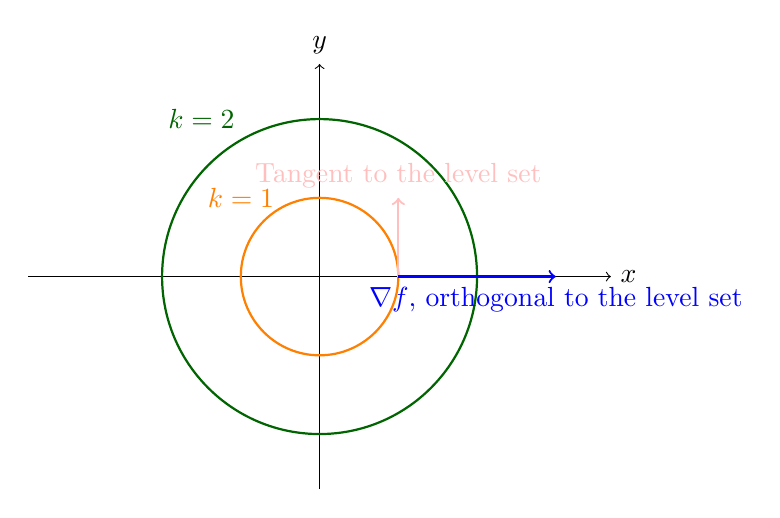
\begin{tikzpicture}
                \draw[->] (-3.7,0) -- (3.7,0) node[right] {$x$};
                \draw[->] (0,-2.7) -- (0,2.7) node[above] {$y$};
                
                \draw[thick,orange] (0,0) circle (1cm);
                \draw[thick,DarkGreen] (0,0) circle(2cm); 
                
                \draw[thick,pink,->] (1,0) -- (1,1) node[above] {Tangent to the level set};
                \draw[thick,blue,->] (1,0) -- (3,0) node[below] {$\nabla f$, orthogonal to the level set};
                
                \node[orange] at (-1,1) {$k=1$};
                \node[DarkGreen] at (-1.5,2) {$k=2$};
            \end{tikzpicture}
    \end{center}
\end{enumerate}

\begin{exercise}
    $f(x, y, z) = e^{2x}y + y^2 + 4$. At the point $(0, 0)$, find the directional derivative along the direction given by $\vec{u} = (1, 3)$ (first turn $\vec{v}$ into a unit vector). 
\end{exercise}

\begin{exercise}
    $f(x, y, z) = x^2y + z$. At the point $(2, 2, 1)$, find the maximum rate of change, and the direction with the maximum (the direction with maximum rate of change is $\nabla f$, and the value of this maximum rate of change is $| \nabla f |$). 
\end{exercise}

\begin{exercise}
    Define $f(x, y, z) = xy^2e^z$. Let $f(x, y, z) = e$. 

    At the point $(1, 1, 1)$, find the equation of the tangent plane.
\end{exercise}

\begin{exercise}
    Find all directional derivatives at $(0, 0)$ (including the partials), if they exist. Is the function \textbf{continuous} at $(0, 0)$?
    \begin{enumerate}[label=\alph*)]
        \item 
        $f(x, y) = \begin{cases}
            \frac{xy}{x^2 + y^2} & (x, y) \neq (0, 0) \\
            0                    & (x, y) = (0, 0)
        \end{cases}$

        \item $f(x, y) = \sqrt{|xy|}$
    \end{enumerate}

    {~~~}

    \textbf{Strategy:}

    When the function has division by $0$, or some other problems at the origin (such as absolute value or square root), we must use the definition of directional derivative, because $f$ \bred{may not be differentiable} at $(0, 0)$ so the formula $\nabla f \cdot \vec{u}$ does not work. Set $\vec{a} = (0, 0)$ and $\vec{u} = (a, b)$ where $a^2 + b^2 = 1$. 
\end{exercise}

\section{Differentiation}

In first year, we defined the tangent line to be $\frac{\text{rise}}{\text{run}}$, and we calculate the limit as the \textit{run} approaches $0$, where the {\color{DarkGreen}secant line} becomes the {\color{orange}tangent line}. This gives the slope of the tangent line of the function at $x = a$.

\begin{center}
    \tikzsetnextfilename{c03s05-f01}%
    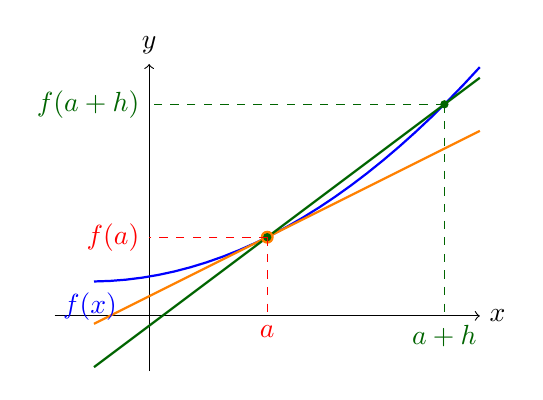
\begin{tikzpicture}
        \draw[->] (-2.7,0) -- (2.7,0) node[right] {$x$};
        \draw[->] (-1.5,-0.7) -- (-1.5,3.2) node[above] {$y$};

        \draw[thick,blue,domain=-2.2:2.7] plot (\x, {(\x/3)^2+(\x/2)+1});

        \draw[thick,orange,domain=-2.2:2.7] plot (\x, {\x/2+1});
        \draw[thick,DarkGreen,domain=-2.2:2.7] plot (\x, {3*\x/4+1});

        \draw[orange,fill=orange] (0,1) circle (0.075cm);
        \draw[DarkGreen,fill=DarkGreen] (0,1) circle (0.045cm);
        \draw[DarkGreen,fill=DarkGreen] (2.25,2.6875) circle (0.045cm);

        \draw[red,dashed] (0,1) -- (0,0) node[below] {$a$};
        \draw[DarkGreen,dashed] (2.25,2.6875) -- (2.25,0) node[below] {$a+h$};
        \draw[red,dashed] (0,1) -- (-1.5,1) node[left] {$f(a)$};
        \draw[DarkGreen,dashed] (2.25,2.6875) -- (-1.5,2.6875) node[left] {$f(a+h)$};

        \node[blue] at (-2.25,0.125) {$f(x)$};
    \end{tikzpicture}
\end{center}

There is another way to interpret the tangent line, however. It is the \itblue{best approximation of the function} using a line. Let $L(x)$ be the equation of the tangent line, and $g(x)$ be the equation of a random line that passes through $(a, f(a))$. Why is $\color{orange} L(x)$ the tangent line and not $\color{DarkGreen}g(x)$?

\begin{center}
    \tikzsetnextfilename{c03s05-f02}%
    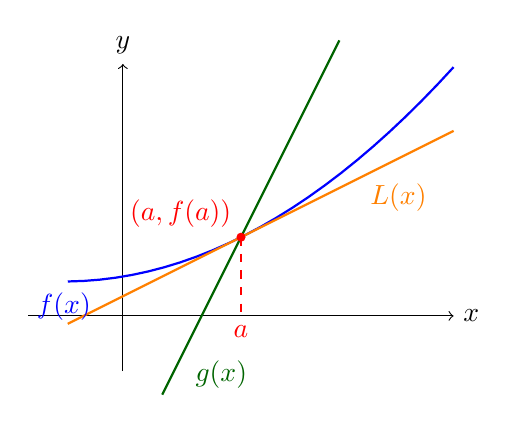
\begin{tikzpicture}
        \draw[->] (-2.7,0) -- (2.7,0) node[right] {$x$};
        \draw[->] (-1.5,-0.7) -- (-1.5,3.2) node[above] {$y$};

        \draw[thick,blue,domain=-2.2:2.7] plot (\x, {(\x/3)^2+(\x/2)+1});

        \draw[thick,orange,domain=-2.2:2.7] plot (\x, {\x/2+1});
        \draw[thick,DarkGreen,domain=-1:1.25] plot (\x, {2*\x+1});

        \draw[red,dashed] (0,1) -- (-0,0) node[below] {$a$};

        \draw[red,fill=red] (0,1) circle (0.05cm) node[above left] {$(a, f(a))$};

        \node[blue] at (-2.25,0.125) {$f(x)$};
        \node[orange] at (2,1.5) {$L(x)$};
        \node[DarkGreen] at (-0.25,-0.75) {$g(x)$};
    \end{tikzpicture}
\end{center}

Clearly, the error made from $L(x)$, $f(x) - L(x)$ goes to $0$ as $x \to a$. However, $\lim_{x\to{a}}g(x)$ is also $0$. It is not sufficient to say that the error goes to $0$, but we also want to check the rate at which the error goes to $0$. So what makes $\color{orange}L(x)$ better than $\color{DarkGreen}g(x)$? While both are approaching $0$, the error for $\color{orange} L(x)$ approaches $0$ \bred{faster} than that of $\color{DarkGreen} g(x)$ \footnote{To denote ``$F(x)$ goes to $0$ faster than $G(x)$'', we use $\lim_{x\to0} \frac{F(x)}{G(x)} = 0$. }. For the tangent line, we want $L(x)$ to approach $f(a)$ the fastest, in particular, faster than how $x$ approached $a$. Thus, we have $\lim_{x\to{a}} \frac{f(x) - L(x)}{x} = 0$.

Recall that the equation of the tangent line is $y - f(a) = f'(a)(x - a)$, so $L(x) = f(a) + f'(a)(x - a)$ \footnote{This is in fact the first order Taylor expansion of $f(x)$ at $a$. }, where $f'(a) = \lim_{h\to0} \frac{f(a+h) - f(a)}{h}$ as before. Take $x = a + h$, we have alternatively
\begin{align*}
    \lim_{h\to0} \frac{f(a + h) - L(a + h)}{h - a}                                       & = 0     \\
    \lim_{h\to0} \frac{f(a + h) - \left[ f(a) + f'(a)(\cancelto{h}{x - a})~~ \right]}{a} & = 0     \\
    \lim_{h\to0} \frac{f(a + h) - f(a)}{h} - \frac{f'(a) \cdot \cancel{h}}{\cancel{h}}   & = 0     \\
    \lim_{h\to0} \frac{f(a + h) - f(a)}{h}                                               & = f'(a)
\end{align*}

This happens to be the equation we have before.

    {~~~}

We can expand this result to higher dimensions. If we have a 2D function, we should have a \term{tangent plane} that allows the error between the function and the tangent plane to approach $0$ faster than any other planes.

Given the tangent plane $w = L(x,y)$, we want $\lim_{\vec{x}\to\vec{a}} f(x,y) - L(x,y) = 0$, and approaches $0$ the fastest. That is, $\lim_{\vec{x}\to\vec{a}} \frac{f(x,y) - L(x,y)}{| \vec{x} - \vec{a} |} = 0$ \footnote{Similar as before, this means we want the error to approach $0$ faster than $\vec{x}$ approaches $\vec{a}$. }.

To get the equation of the tangent plane, we can think of the original function, $f(x,y)$, as the level set of the 3D function $F(x,y,z) = f(x,y) - z$ at $k = 0$. Then, by the result from the previous section, $\nabla F(x_0,y_0,z_0)$ is the normal vector to the tangent plane at the given point $(x_0,y_0,z_0)$. That is, $\vec{n} = \nabla F = \left( \frac{\partial F}{\partial x}, \frac{\partial F}{\partial y}, \frac{\partial F}{\partial z} \right) = \left( \frac{\partial f}{\partial x}, \frac{\partial f}{\partial y}, -1 \right)$.

Note that at $\vec{a} = (x_0, y_0)$, we obtain the point $(x_0, y_0, f(\vec{a}))$ on the graph of $f(x,y)$. Denote this point $\vec{r}_0$, and this allows us to get the formula for the tangent plane.
\begin{align*}
    \vec{n} \cdot \vec{r}
     & = \vec{n} \cdot \vec{r}_0 \\
    \left( \frac{\partial f}{\partial x}, \frac{\partial f}{\partial y}, -1 \right) \cdot \vec{r}
     & = \left( \frac{\partial f}{\partial x}, \frac{\partial f}{\partial y}, -1 \right) \cdot \left( x_0, y_0, f(\vec{a}) \right) \\
    \frac{\partial f}{\partial x} \cdot x + \frac{\partial f}{\partial y} \cdot y - z
     & = \frac{\partial f}{\partial x} \cdot x_0 + \frac{\partial f}{\partial y} \cdot y_0 - f(\vec{a}) \\
    z
     & = f(\vec{a}) + \frac{\partial f}{\partial x} (x - x_0) + \frac{\partial f}{\partial y} (y - y_0) \\
    z
     & = f(\vec{a}) + \nabla f(\vec{a}) \cdot (x-x_0, y-y_0)
\end{align*}

To further simplify this equation, take $(x,y) = \vec{x} = \vec{a} + \vec{h}$. Then, $\vec{h} = \vec{x} - \vec{a} = (x - x_0, y - y_0)$. Now, $z = f(\vec{a}) + \nabla f(\vec{a}) \cdot \vec{h}$.

Substitute the equation for $L(x,y)$ back into $\lim_{\vec{x}\to\vec{a}} \frac{f(x,y) - L(x,y)}{| \vec{x} - \vec{a} |} = 0$, we obtain
\begin{align*}
    \lim_{\vec{x}\to\vec{a}} \frac{f(x,y) - L(x,y)}{| \vec{x} - \vec{a} |}
     & = 0 \\
    \lim_{\vec{h}\to\vec{0}} \frac{f(\vec{a} + \vec{h}) - \left( f(\vec{a}) + \nabla f(\vec{a}) \cdot \vec{h} \right)}{| \vec{h} |}
     & = 0 \\
    \lim_{\vec{h}\to\vec{0}} \frac{f(\vec{a} + \vec{h}) - f(\vec{a}) - \nabla f(\vec{a}) \cdot \vec{h}}{| \vec{h} |}
     & = 0
\end{align*}

\begin{definition}[Differentiable]\index{Differentiable}
    $f$ is \term{differentiable} if the gradient vector $\nabla f(\vec{a})$ satisfies $$\lim_{\vec{h} \to \vec{0}} = \frac{f(\vec{a} + \vec{h}) - f(\vec{a}) - \nabla f(\vec{a}) \cdot \vec{h}}{| \vec{h} |} = 0$$
\end{definition}

Note that this is a \itblue{2D limit}. This limit is typically used when $\vec{a} = (0, 0)$, so we may set $\vec{h} = (x, y)$ and show the limit is zero using Squeeze Theorem.

{~~~}

Some useful facts:

\begin{enumerate}
    \item If $f$ is $C^1$ at $\vec{a}$ \footnote{This means all partial derivatives exist near $\vec{a}$ and at $\vec{a}$, and the partial derivatives are \bred{continuous} (as functions) at $\vec{a}$. }, then $f$ is differentiable at $\vec{a}$ ($\nabla f$ exists). 

    \item Being differentiable is a stronger condition than having directional derivative. If $f$ is differentiable, then all directional derivative is given by $D_{\vec{u}} f = \nabla f \cdot \vec{u}$. 

    \item If a function $f$ is differentiable at $\vec{a}$, then $f$ is continuous at $\vec{a}$.
\end{enumerate}

{~~~}

\begin{exercise}
    Define $$f(x, y) = \begin{cases}
        \frac{xy}{x^2 + y^2} & (x, y) \neq (0, 0) \\
        0                    & (x, y) = (0, 0)
    \end{cases}$$

    Show the directional derivatives exist at $(0, 0)$, but $f$ is \textbf{not differentiable} at $(0, 0)$.

    {~~~}

    \textbf{Strategy:}
    
    There are 2 ways to approach the problem.

    \begin{enumerate}
        \item If the function is \textbf{not continuous} at $(0, 0)$, then it is \textbf{not differentiable} at $(0, 0)$. So we may try to show it is not continuous at $(0, 0)$. However, some functions \textbf{are continuous} at $(0, 0)$, so we can attain no conclusion in such cases.

        \item Compute all the directional derivatives. If $f$ is differentiable, then every directional derivative should satisfy $D_{\vec{u}} f = \nabla f \cdot \vec{u}$. 
        
        Check this equation for $\vec{u} = (1, 0)$, $\vec{u} = (0, 1)$, and $\vec{u} = \left( \frac{1}{\sqrt{2}}, \frac{1}{\sqrt{2}} \right)$ (easy unit vectors). 
    \end{enumerate}
\end{exercise}

\begin{exercise}
    Show whether the function is differentiable at $(0, 0)$.

    \begin{enumerate}[label=\alph*)]
        \item $f(x, y) = \begin{cases}
            \frac{x|y|}{\sqrt{x^2 + y^2}} & (x, y) \neq (0, 0) \\
            0                             & (x, y) = (0, 0)
        \end{cases}$

        \item $f(x, y) = \begin{cases}
            \frac{x^4 + y^4}{x^2 + y^2} & (x, y) \neq (0, 0) \\
            0                           & (x, y) = (0, 0)
        \end{cases}$
    \end{enumerate}
\end{exercise}

\section{Higher Order Derivative}

We may take (partial) derivatives on top of partial derivatives. 

In 2 dimensions, for $f(x, y)$, there are 4 ways of taking second derivatives. We put them into the \term{Hessian Matrix}\index{Hessian Matrix}: 
$$H = \begin{bmatrix}
    \frac{\partial^2 f}{\partial x^2} & \frac{\partial^2 f}{\partial xy}  \\
    \frac{\partial^2 f}{\partial yx}  & \frac{\partial^2 f}{\partial y^2}
\end{bmatrix} = \begin{bmatrix}
    \frac{\partial f}{\partial x}\left( \frac{\partial f}{\partial x} \right) & 
    \frac{\partial f}{\partial x}\left( \frac{\partial f}{\partial y} \right)   \\
    \frac{\partial f}{\partial y}\left( \frac{\partial f}{\partial x} \right) & 
    \frac{\partial f}{\partial y}\left( \frac{\partial f}{\partial y} \right)
\end{bmatrix} = \begin{bmatrix}
    f_{xx} & f_{xy} \\ f_{yx} & f_{yy}
\end{bmatrix}$$

{~~~}

If $f$ is $C^2$ at $\vec{a}$ \footnote{This means all the 2nd order partial derivatives exist near $\vec{a}$ and at $\vec{a}$, and the 2nd order partial derivatives are continuous (as functions) at $\vec{a}$ (In practice, a function can fail to be continuous when there is division by zero). }, then \bred{mixed partial derivatives commute}:

The order of taking derivatives does not change the final answer: $f_{xy} = f_{yx} \to$ Taking derivative in $x$ then $y$ is the same as taking in $y$ then $x$.

In other words, if $f$ is $C^2$, then \bred{the Hessian Matrix is symmetric}.

{~~~}

We can also construct the Hessian for $f(x, y, z)$, which will be a $3 \times 3$ matrix. We can also construct higher order derivatives, such as 3rd order $f_{xyz}$ or $f_{xyy}$. In general, if $f$ is $C^k$, then mixed partial derivatives commute (up to order $k$).

\begin{exercise}
    Find the Hessian Matrix.

    \begin{minipage}[t]{0.45\linewidth} \setstretch{1.5}
        \begin{enumerate}
            \item $f(x, y) = 3x^2 + 4xy + 5y^2$
            \item $f(x, y) = \cos(x + 2y)$
            \item $f(x, y) = x^{2x + y}$
        \end{enumerate}
    \end{minipage}
    \begin{minipage}[t]{0.45\linewidth} \setstretch{1.5}
        \begin{enumerate} \setcounter{enumi}{3}
            \item $f(x, y) = e^{x^2 + y}$
            \item $f(x, y) = e^x \sin(y)$
            \item $f(x, y, z) = x^2y + xz + z^2$
        \end{enumerate}
    \end{minipage}
\end{exercise}

\begin{exercise}
    $$f(x, y) = \begin{cases}
        \frac{x^3y - xy^3}{x^2 + y^2} & (x, y) \neq (0, 0) \\
        0                             & (x, y) = (0, 0)
    \end{cases}$$

    Find $f_x$ and $f_y$ at $(x, y) = (0, 0)$ \textbf{and} $(x, y) \neq (0, 0)$. Then show $f_{xy} \neq f_{yx}$ at $(0, 0)$. i.e. Taking 2nd derivatives in different orders give different answers. 

    Is $f$ $C^2$ at $(0, 0)$ (and have we reacher a contradiction)?
\end{exercise}

\section{Critical Points}

In first year, we found critical points of functions by setting the derivative to zero. Then we check their second derivative to conclude whether critical points are max or min. In higher dimensions, it is very similar.

Let $f(x, y)$ be a 2D function (which is $C^2$).

We set $\nabla f(\vec{x}) = \vec{0}$. Solve $\vec{x}$, these are the \term{critical points}\index{Crtitial Point}.

Then we check second derivatives: \bred{the Hessian Matrix}.
$$H = \begin{bmatrix}
    \frac{\partial^2 f}{\partial x^2} & \frac{\partial^2 f}{\partial xy}  \\
    \frac{\partial^2 f}{\partial yx}  & \frac{\partial^2 f}{\partial y^2}
\end{bmatrix}$$

Note that $H$ can contain $x$ and $y$, so $H$ would be different for different points. For each critical point $\vec{a}$, 
\begin{itemize}
    \item if $\det(H(\vec{a})) > 0$, look at the top left entry
    
    \begin{itemize}
        \item if $\frac{\partial^2 f}{\partial x^2}(\vec{a}) > 0$,  then it is a \term{local minimum}\index{Local Minimum}.
        \item if $\frac{\partial^2 f}{\partial x^2}(\vec{a}) < 0$,  then it is a \term{local maximum}\index{Local Maximum}.
    \end{itemize}

    \item if $\det(H(\vec{a})) < 0$, it is a \term{saddle point}\index{Saddle Point}. 

    \item if $\det(H(\vec{a})) = 0$, it is inconclusive. 
\end{itemize}

To find the (absolute) maximum and minimum of $f$ in a region $D$, 
\begin{enumerate}
    \item Find all local extrema inside $D$ using critical points
    \item Find all extrema on the \bred{boundary} of $D$ 
    \item Compare all the function values to attain the absolute extrema
\end{enumerate}

\begin{exercise}
    Find and classify all critical points.

    \begin{enumerate}
        \item $f(x,y) = 3x^2 + 2xy + 5y^2$
        \item $f(x,y) = x^2 + 3y^4 + 4y^3 - 12y^2$
        \item $f(x,y) = (x - 1)(x^2 + y^2)$
        \item $f(x,y) = (x^2 + 2y^2)e^{-x^2 - y^2}$
    \end{enumerate}
\end{exercise}

\begin{exercise}
    Let $f(x,y) = x^2 + y^2 - 4x$

    Find the max and min indide the triangle $D$ defined by $(0, -3)$, $(0, 3)$, and $(3, 0)$. 
\end{exercise}

\section{Lagrange Multiplier}

Sometimes, we want to maximim/minimize a function on some specific curve, or there are some constraints on the variables that the function takes in. 

\begin{itemize}
    \item Take the function we want to maximize/minimize to be $f$.

    \item Take the equation that describes the constraint to be $g = 0$ (perhaps we have more than 1 constraint, so the second constraint is $h = 0$).

    \item The \term{Lagrange Multiplier Formula}\index{Lagrange Multiplier Formula} is $$\nabla f = \lambda \nabla g(+\mu \nabla h + \cdots)$$
\end{itemize}

Each constraint will create an extra $\nabla$ term on the right side with some constant in front (we need every $\nabla$ term on the right to be non-zero). 

$\lambda$ and $\mu$ are constants that you need to solve for, along with $n$ variables of $f$. The equation is an equation for vectors, so each of the components are equal. So, there are $n$ equations in the formula since $\nabla f$ has $n$ components. For each constant like $\lambda$ or $\mu$, there is a equation of constraint for each. So if there are 2 constraints, there are $n + 2$ variables that you need to solve, and you have $n + 2$ equations to do it.

You are \bred{not allowed to divide by zero} when you cancel terms. When attempting to divide a quantity $x$, you need to split into 2 cases:
\begin{itemize}
    \item When $x \neq 0$, you can divide
    \item when $x = 0$, you cannot
\end{itemize}

\begin{exercise}
    Find the max and min of the function $f(x, y)$ subject to constraints given.

    $f(x,y) = 2x - 6y$ with constraint $4x^2 + 2y^2 = 25$. 
\end{exercise}

\begin{exercise}
    Consider the curve in $\mathbb{R}^2$, $C: y = x^2$. 

    Find the point $p$ on $C$ so that the distance between $p$ and $(0, -1)$ is smallest.

    \textbf{Strategy}: We minimize $f(x, y) = \text{distance}^2 = (x - 0)^2 + (y -(-1))^2$.
\end{exercise}

\begin{exercise}
    Consider 2 curves in $\mathbb{R}^2$, $C_1: y = x^2$ and $C_2: y = x - 1$

    Find points $p$ on $C_1$ and $q$ on $C_2$ so that the distance between them is smallest.
\end{exercise}

\section{Chain Rule in 1D}

We typically think of chain rule as a rule for computation: $$f(g(x))' = f'(g(x)) \cdot g'(x)$$ where we are given a function inside another function such as $y = \sin(e^x)$, and we take the derivative of the outside (not touching the inside), then multiply the derivative of the inside.

Alternatively, we can define a \bred{variable dependence}. For example, define the variables as $y = y(t)$, and $t = t(x)$. (In the above example, we would set $y = \sin t$ and $t = e^x$.) Then we may express the chain rule (in 1D) as: $$\frac{dy}{dx} = \frac{dy}{dt} \frac{dt}{dx}$$

Intuitively, $\frac{dy}{dx}$ asks how much would $y$ change, if there is a small change in $x$. Given the variable dependence above, a small change in $x$ would cause a small change in $t$, which in turn would cause a small change in $y$. Hence, we have the 2 ``fractions'' ($\frac{dy}{dt}$ and $\frac{dt}{dx}$) on the right.

\subsection*{2nd Derivative}

We may use the above form of the chain rule to calculate the 2nd derivative.

We apply another differential operator $\frac{d}{dx}$ on top of $\frac{dy}{dx}$: $$\frac{d^2y}{dx^2} = \frac{d}{dx} \left( \frac{dy}{dx} \right)$$ Plug in the above form of the chain rule, $$= \frac{d}{dy} \left( \frac{dy}{dt} \frac{dt}{dx} \right)$$ We want to take the derivative of this product, so we need \term{product rule}\index{Product Rule (in 1D)}, $$= \frac{d}{dx}\left( \frac{dy}{dt} \right) \cdot \frac{dt}{dx} + \frac{dy}{dt} \cdot \frac{d}{dx} \left( \frac{dt}{dx} \right)$$ Notice that there are 2 types of derivatives here.

{~~~}

The 2nd term involves the expression $\frac{d}{dx} \left( \frac{dt}{dy} \right)$. Recall that we assumed $t = t(x)$ (such as $t = e^x$), so $\frac{dt}{dx}$ is also \bred{a function of $x$}. We want to take the derivative of such function \bred{against $x$}. This results in the 2nd derivative of $t = t(x)$ against $x$: $$\frac{d}{dx} \left( \frac{dt}{dx} \right) = \frac{d^2t}{dx^2}$$ The 1st term involves the expression $$\frac{d}{dx} \left( \frac{dy}{dt} \right)$$ This term is more difficult (and requires an \bred{additional expansion}). 

Recall that we assumed y = y(t) (such as y = sin t), so $\frac{dy}{dt}$ is also \bred{a function of $t$} (such as $dy = \cos t$). 

We want to take the derivative of such function \bred{against $x$}, on an expression involving $t$.

{~~~}

Notice that $\frac{dy}{dt}$ is an expression involving t, similar to $y = y(t)$. So to take the derivative against $x$, on an expression involving $t$, we know that for $y = y(t)$: $$\frac{d}{dx} \left( y(t) \right) = \frac{dy}{dx} = \frac{dy}{dt} \frac{dt}{dx} = \frac{d}{dx} \left( y(t) \right) \frac{dt}{dx}$$ Since $\frac{dy}{dt}$ is also an expression involving t, it would \bred{behave in the same way} as $y(t)$ when taking derivative \bred{against $x$}.

We can substitute $y(t)$ with $\frac{dy}{dx}$ in the above expression: $$\frac{d}{dx} \left( \frac{dy}{dt} \right) = \frac{d^2y}{dt^2}$$ 

In conclusion, to take \bred{the 2nd derivative involving chain rule}: $$\frac{d^2y}{dx^2} = \frac{d}{dx} \left( \frac{dy}{dx} \right) = \frac{d}{dx} \left( \frac{dy}{dt} \frac{dt}{dx} \right) = \frac{d}{dx} \left( \frac{dy}{dt} \right) \cdot \frac{dt}{dx} + \frac{dy}{dt} \cdot \frac{d}{dx} \left( \frac{dt}{dx} \right)$$ Taking an \bred{additional expansion} in the first term: 
$$\begin{aligned}[t]
    & = \frac{d}{dt} \left( \frac{dy}{dt} \right) \frac{dt}{dx} \cdot \frac{dt}{dx} + \frac{dy}{dt} \cdot \frac{d^2t}{dx^2} \\ 
    & = \frac{d^2y}{dt^2} \frac{dt}{dx} \cdot \frac{dt}{dx} + \frac{dy}{dt} \cdot \frac{d^2t}{dx^2}
\end{aligned}$$

Notice that we get a square of $\frac{dt}{dx}$ in the first term. Thus \bred{the chain rule formula for 2nd derivative} is: $$\frac{d^2y}{dx^2} = \frac{d^2y}{dt^2} \left( \frac{dt}{dx} \right)^2 + \frac{dy}{dt} \cdot \frac{d^2t}{dx^2} \footnote{Note $\left( \frac{dt}{dx} \right)^2 \neq \frac{d^2t}{dx^2}$. }$$ 

Of course, given a function $y = y(x)$, one would not go through this long and complicated process just to take 2nd derivative. It is much easier to just take the derivative (twice) using the computation rules.

However, this formula shines when \bred{at least one of the function is unknown}. This is exactly the case for \bred{ODE}, where $y = y(x)$ is unknown. We may use this formula to carry out a \bred{change of variables} and turn a complicated ODE into a simple one.

\subsection*{ODE - Euler Equation}

Consider $y = y(x)$. For numbers $a$, $b$, $c$, $$ax^2y'' + bxy' + cy = 0$$ This is a \term{2nd order linear equation}\index{2nd Order Linear Equation}, but with non-constant coefficients. In general, this type of equation has no solution. But here, notice that we have exactly $x^2$ in front of $y''$, and $x$ in front of $y'$.

Due to this, we can guess the solution to be $y(x) = x^n$. We plug in $y(x) = x^n$ into the ODE, and solve for $n$.

{~~~}

Typically, there will be 2 solutions for $n$. The general solution will be a linear combination of the 2 solutions (with constants $c1$ ,$c2$ in front).

\begin{example}
    $$x^2y'' - xy' - 3y = 0$$

    Take $y = x^n$, then $y' = nx^{n-1}$ and $y'' = n(n - 1)x^{n-2}$.

    Plugging into the ODE, $$x^2 n(n - 1) x^{n-2} - x n x^{n-1} - 3x^n = 0$$

    Notice that we can divide both sides by $x^n$.
    $$\begin{aligned}[t]
        n(n - 1) - n - 3 & = 0 \\
        n^2 - 2n - 3     & = 0
    \end{aligned}$$ 

    We will always get a quadratic of this form. In this case, we get $$(n - 3)(n + 1) = 0$$

    Thus the general solution is given by $$y(x) = c_1x^3 +c_2^{-1}$$
\end{example}

However, notice that given an equation with different numbers, the quadratic we get may have only one (repeated) solution. In this case, we would be ``missing'' the second solution. We can instead find the solution by using the chain rule formula for 2nd derivative. 

\begin{example}
    $$x^2y'' - 3xy' + 4y = 0$$

    If we proceed using the previous approach, we would get $(n - 2)^2 = 0$, giving one (repeated) solution.

    Instead, we can perform a change of variable, $t = \ln x$. We get 

    \begin{minipage}[t]{0.45\linewidth}
        \begin{align*}
            y' = \frac{dy}{dx} & = \frac{dy}{dt} \frac{dt}{dx} \\
                               & = \frac{dy}{dt} \frac{1}{x}
        \end{align*}
    \end{minipage}
    \begin{minipage}[t]{0.45\linewidth}
        \begin{align*}
            y'' & = \frac{d^2y}{dt^2} \left( \frac{dt}{dx} \right)^2 + \frac{dy}{dt} \cdot \frac{d^2t}{dx^2} \\
                & = \frac{d^2y}{dt^2} \left( \frac{1}{x} \right)^2 + \frac{dy}{dt} \cdot \frac{-1}{x^2}
        \end{align*}
    \end{minipage}

    Plugging the above into the ODE,
    $$\begin{aligned}[t]
        x^2y'' - 3xy' + 4y & = 0 \\
        x^2 \left( \frac{d^2y}{dt^2} \left( \frac{1}{x} \right)^2 + \frac{dy}{dt} \cdot \frac{-1}{x^2} \right) - 3x \left( \frac{dy}{dt} \frac{1}{x} \right) + 4y &= 0
    \end{aligned}$$

    Notice that all the $x$ cancels out.
    $$\begin{aligned}[t]
        \frac{d^2y}{dt^2} - \frac{dy}{dt} - 3\frac{dy}{dt} + 4y & = 0 \\
        \frac{d^2y}{dt^2} - 4\frac{dy}{dt} + 4y                 & = 0
    \end{aligned}$$

    This is a \itblue{2nd order linear equation with constant coefficients}. The solution is given by $y(t) = e^{rt}$.

    Plugging into the equation, 
    $$\begin{aligned}[t]
        r^2 - 4r + 4 & = 0 \\ 
        (r - 2)^2    & = 0
    \end{aligned}$$

    This is a \bred{repeated} root solution. Thus the general solution for $y(t)$ is given by $$y(t) = c_1 e^{2t} + c_2 t e^{2t}$$

    Since $t = \ln{x}$, we get the general solution for $y(x)$ is given by 
    $$\begin{aligned}[t]
        y(t) & = c_1 e^{2 \ln{x}} + c_2 \ln{x} e^{2 \ln{x}}                               \\
             & = c_1 \left( e^{\ln{x}} \right)^2 + c_2 \ln{x} \left( e^{\ln{x}} \right)^2 \\
             & = c_1 x^2 + c_2 (\ln{x}) x^2
    \end{aligned}$$
\end{example}

In other words, the ``missing'' second solution from the repeated root of $n = 2$, is attained by multiplying an extra factor of $\ln{x}$ in front of $x^n$.

\begin{exercise}
    Find the general solution to the ODE, where $y = y(x)$.

    {~~~}

    \begin{enumerate}
        \item $x^2y'' - 3xy' + 4y = 0$
        \item $2x^2y'' - 5xy' + 5y = 0$
        \item $x(1 - x^2)^2y'' - (1 - x^2)(1 + 4x^2)y' + 2x^3y = 0$ with the change of variable $t = \frac{-1}{2} \ln(1 - x^2)$
    \end{enumerate}
\end{exercise}

\section{Chain Rule in 2D and 3D}

Consider an example: $\begin{cases}z = z(x, y) \\ x = x(s, t) \\ y = y(s, t) \end{cases}$. We can construct the tree diagram of variable dependence.

\begin{center}
    \tikzsetnextfilename{c03s10-f01}%
    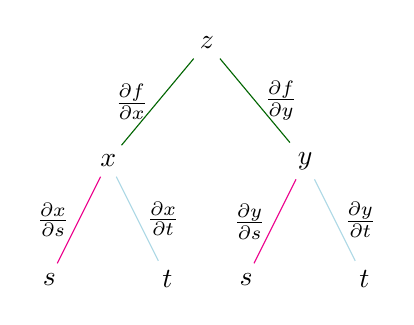
\begin{tikzpicture}[
        level 1/.style = {sibling distance = 2.5cm},
        level 2/.style = {sibling distance = 1.5cm}
    ]
    
    \node {$z$} 
        child {
            node {$x$}
            child {
                node [black] {$s$}
                edge from parent [magenta] node [left,black] {{$\frac{\partial x}{\partial s}$}}
            }
            child {
                node [black] {$t$}
                edge from parent [LightBlue] node [right,black] {{$\frac{\partial x}{\partial t}$}}
            }
            edge from parent [DarkGreen] node [left,black] {{$\frac{\partial f}{\partial x}$}}
        }
        child {
            node {$y$}
            child {
                node [black] {$s$}
                edge from parent [magenta] node [left,black] {{$\frac{\partial y}{\partial s}$}}
            }
            child {
                node [black] {$t$}
                edge from parent [LightBlue] node [right,black] {{$\frac{\partial y}{\partial t}$}}
            }
            edge from parent [DarkGreen] node [right,black] {$\frac{\partial f}{\partial y}$}
        };
    \end{tikzpicture}
\end{center}

We start with the variable $z$ on the top, and for each variable that $z$ depends on, we get an extra branch below. In this case, $z = z(x, y)$ and we get 2 branches for $x$ and $y$. The 2 branches correspond to the partial derivatives $\frac{\partial z}{\partial x}$ and $\frac{\partial f}{\partial z}$ as we will see. 

Similarly, we create branches for x and y, and get 4 branches for $s$ and $t$. The branches correspond to the partial derivatives $\frac{\partial x}{\partial s}$, $\frac{\partial x}{\partial t}$, $\frac{\partial y}{\partial s}$ and $\frac{\partial y}{\partial t}$. 

To compute $\frac{\partial z}{\partial s}$, using the diagram, we start at $z$, and \bred{consider all possible ways to reach $s$}. The first way is, start from $z$, go to $x$, then from $x$ to $s$. This gives (using multiply) $$\frac{\partial z}{\partial x} \cdot \frac{\partial x}{\partial s}$$ 

The second way is, start from $z$, go to $y$, then from $y$ to $s$. This gives (using multiply) $$\frac{\partial z}{\partial y} \cdot \frac{\partial y}{\partial s}$$

The answer is the 2 ways \bred{added together}, $$\frac{\partial z}{\partial s} = \frac{\partial z}{\partial x} \cdot \frac{\partial x}{\partial s} + \frac{\partial z}{\partial y} \cdot \frac{\partial y}{\partial s}$$

Similarly, $$\frac{\partial z}{\partial t} = \frac{\partial z}{\partial x} \cdot \frac{\partial x}{\partial t} + \frac{\partial z}{\partial y} \cdot \frac{\partial y}{\partial t}$$

Intuitively, $\frac{\partial z}{\partial s}$ asks how much would $z$ change, if there is a small change in $s$. Given the variable dependence above, a small change in $s$ would cause both a small change in $x$ and a small change in $y$. The small change in $x$ would in turn cause a small change in $z$, and the the small change in $y$ would also cause a small change in $z$. Thus the ``total'' small change in $z$ would be the sum of the 2 changes caused by $x$ and $y$. Hence, we get the sum of 2 pairs of ``fractions'' multiplied on the right.

Of course, given the functions $z = z(x, y)$ and $x = x(s, t)$, $y = y(s, t)$, one does not need go through this long and complicated process just to take the derivative. It is much easier to just plug in the expression of $x$ and $y$ into $z$, and take the derivative using the computation rules.

\begin{exercise}
$\text{ }$

    \begin{enumerate}
        \item $z = x - y$, $x = \sin(t)$, $y = 3t$. Find $\frac{\partial z}{\partial t}$.
        \item $z = xy^2$, $x = s\cos(t)$, $y = s\sin(t)$. Find $\frac{\partial z}{\partial x}$ and $\frac{\partial z}{\partial t}$.
        \item $u = xy + yz$, $x = s + t$, $y = s$, $z = 2t$. Find $\frac{\partial u}{\partial s}$ and $\frac{\partial u}{\partial t}$.
    \end{enumerate}
\end{exercise}

Similar to the Chain Rule in 1D, the chain rule formula shines when \bred{at least one of the function} is unknown.

\begin{exercise}
    Suppose that $z = f(x, y)$, $x = 2s + t$ and $y = s - 3t$. Assume $f(1,1) = 2$, $f(3,-2) = 1$, $z_x(1,1) = 2$, $z_x(3,-2) = 4$, $z_y(1,1) = 6$, and $z_y(3,-2) = 1$. Find $z_s$ and $z_t$ at $(s,t) = (1,1)$.
\end{exercise}

\subsection*{PDE - Partial Differential Equation}

A \term{Partial Differential Equation (PDE)}\index{Partial Differential Equation (PDE)} is an equation, which implicitly defines a function $u(x, y)$ by mixing $u$, $x$, $y$, and \itblue{(partial) derivatives of $u$}.

Similar to ODE, the function $u(x, y)$ defined by an PDE often can not be solved explicitly. Different from an ODE, the general solution of a PDE would involves some \itblue{unknown function}, instead of unknown constants.

\subsection*{First Order Linear Equation with Constant Coefficients}

Consider $u = u(x, y)$. Consider the example $$2u_x + 3u_y = 0$$

We perform the change of variables $s = 2x + 3y$ and $t = 3x - 2y$. (This change of variable works in general: $a = 2$, and $b = 3$ in this case \footnote{In general, for $au_x + bu_y$, we would set $s = ax + by$ and $t = bx - ay$. }.) Using chain rule (where we think of $u$ as $u = u(s,t)$, $s = s(x,y)$, $t = t(x,y)$), 
$$\begin{aligned}[t]
    \frac{\partial u}{\partial x}
     & = \frac{\partial u}{\partial s} \cdot \frac{\partial s}{\partial x} + \frac{\partial u}{\partial t} \cdot \frac{\partial t}{\partial x} \\
     & = \frac{\partial u}{\partial s} \cdot 2 + \frac{\partial u}{\partial t} \cdot 3 \\
    \frac{\partial u}{\partial y}
     & =  \frac{\partial u}{\partial s} \cdot \frac{\partial s}{\partial y} + \frac{\partial u}{\partial t} \cdot \frac{\partial t}{\partial y} \\
     & = \frac{\partial u}{\partial s} \cdot 3 + \frac{\partial u}{\partial t} \cdot (-2)
\end{aligned}$$

Plugging into the PDE, we get 
$$\begin{aligned}[t]
    2u_x + 3u_y & = 0 \\
    2 \left( \frac{\partial u}{\partial s} \cdot 2 + \frac{\partial u}{\partial t} \cdot 3 \right) + 3 \left( \frac{\partial u}{\partial s} \cdot 3 + \frac{\partial u}{\partial t} \cdot (-2) \right) & = 0
\end{aligned}$$

Notice that the terms involving $\frac{\partial u}{\partial t}$ cancels. $$(2^2 + 3^2) \frac{\partial u}{\partial s} = 0$$ Thus the partial derivative of $u(s, t)$ against $s$ is $0$. 

However, since we are in 2D, this does not mean $u$ is constant. For example, $u(s, t) = t^2$, would have $\frac{\partial u}{\partial s} = 0$, which implies that $u$ must \bred{not} depend on $s$, but can still depend on $t$. To signal this dependence, we get $$u(s, t) = f(t)$$ where $f$ is a 1D function only depending on $t$. 

Since $t = 3x - 2y$, the \bred{general solution} of $u$ is given by $$u(x, y) = f(3x - 2y)$$ Notice that the general solution involves an \bred{unknown function} $f$.

\subsection*{Initial Condition}

Indeed, one may check that $u(x, y) = f (3x - 2y)$ satisfy the original PDE, without needing to know what the unknown function $f$ is.

However, one may impose an \bred{initial condition} on $u$, which would allow one to solve for $f$. This is analogous to imposing an initial condition on an ODE, which would solve for the constants.

Suppose in the above example, we impose the initial condition: $u(x, 0) = x^2$. Then since the general solution is $u(x, y) = f(3x - 2y)$: $$u(x,0) = f(3x) = x^2$$

We may solve for $f$ by taking a substitution $w = 3x$, so $x = \frac{w}{3}$. $$f(w) = \frac{w^2}{9}$$ 

Thus, the \bred{particular solution} is $$u(x,y) = f(3x-2y) = \frac{(3x-2y)^2}{9}$$

\subsection*{General Case}

For the equation $au_x +bu_y = 0$, set $s = ax + by$ and $t = bx - ay$. The \bred{general solution} is $u(x, y) = f (bx - ay)$.

\begin{exercise}
    Consider $u = u(x, y)$. Find the solution to the PDE (general or particular). 

    \begin{enumerate}
        \item $-u_x + u_y = 0$ with $u(x, 0) = x$.
        \item $au_x + bu_y = 0$.
        \item $u_x + u_y = 1$.
        \item $u_x - u_y + u = 0$.
        \item $u_x + u_y + u = e^{x+2y}$ with $u(x, 0) = 0$. 
        \item $u_x + 2u_y +(2x - y)u = 2x^2 +3xy - 2y^2$.
    \end{enumerate}
\end{exercise}

\begin{exercise}
    Consider $2u_x + yu_y = 0$.

    (First order linear equation with non-constant coefficients: $a = 2$, $b = y$) 

    Find the solution with the change of variables $s = x$, $t = e^{-\frac{x}{2y}}$.

    ($C = e^{-\frac{x}{2y}}$ is the solution to the ODE: $\frac{dy}{dx} = \frac{y}{2} = \frac{b}{a}$)
\end{exercise}

\section{Higher Order Chain Rule}

Chain rule with higher order derivatives are very complicated. 

Consider a simple example, $u = u(x, y)$, $x = x(s, t)$ and $y = y(s, t)$. 

Using the 1st order chain rule, $$\frac{\partial u}{\partial t} = \frac{\partial u}{\partial x} \cdot \frac{\partial x}{\partial t} + \frac{\partial u}{\partial y} \cdot \frac{\partial y}{\partial t}$$ then we can apply another differential operator to attain a second derivative, we use product rule, $$\begin{aligned}[t]
    \frac{\partial}{\partial t}\left(\frac{\partial u}{\partial t}\right) & = \frac{\partial}{\partial t} \left( \frac{\partial u}{\partial x} \cdot \frac{\partial x}{\partial t} \right) + \frac{\partial}{\partial t}\left( \frac{\partial u}{\partial y} \cdot \frac{\partial y}{\partial t} \right) \\
     & = \frac{\partial}{\partial t} \left( \frac{\partial u}{\partial x} \right) \cdot \frac{\partial x}{\partial t} + \frac{\partial u}{\partial x} \cdot \frac{\partial}{\partial t}\left( \frac{\partial x}{\partial t} \right) + \frac{\partial}{\partial t} \left( \frac{\partial u}{\partial y} \right) \cdot \frac{\partial y}{\partial t} + \frac{\partial u}{\partial y} \cdot \frac{\partial }{\partial t} \left( \frac{\partial y}{\partial t} \right)
\end{aligned}$$

Since $u = u(x, y)$, $\frac{\partial u}{\partial x}$ and $\frac{\partial u}{\partial y}$ are \bred{also} functions of $x$ and $y$, so we use the 1st order chain rule from above, except we \bred{replace} u with $\frac{\partial u}{\partial x}$ and $\frac{\partial u}{\partial y}$: 
$$ \frac{\partial}{\partial t} \left(\frac{\partial u}{\partial x} \right) = \frac{\partial}{\partial x} \left( \frac{\partial u}{\partial x} \right) \frac{\partial x}{\partial t} + \frac{\partial}{\partial y} \left( \frac{\partial u}{\partial x} \right) \frac{\partial y}{\partial t}$$
$$ \frac{\partial}{\partial y} \left(\frac{\partial u}{\partial y} \right) = \frac{\partial}{\partial x} \left( \frac{\partial u}{\partial y} \right) \frac{\partial x}{\partial t} + \frac{\partial}{\partial y} \left( \frac{\partial u}{\partial y} \right) \frac{\partial y}{\partial t}$$

These 2 expressions go into the above formula and give a total of 6 terms of $\frac{\partial}{\partial t} \left( \frac{\partial u}{\partial t} \right)$. 

\begin{exercise}
    Let $u = u(x, y)$, $x = st + t^2$ and $y = se^t$. Find $\frac{\partial^2 u}{\partial s \partial t}$. 
\end{exercise}

\begin{exercise}
    We find the general solution $u = u(x, t)$ to the PDE, the \textbf{wave equation}: $$u_{tt} - c^2u_{xx} = 0$$ where $c$ is a constant, called the ``speed of the wave''. 

    We consider the \textbf{change of variables} $v = x+ct$ and $w = x-ct$. 

    \begin{enumerate}
        \item Find $u_t$ and $u_x$, according to the change of variables given. 
        \item Find $u_{tt}$ and $u_{xx}$. 
        \item Find the \textbf{general solution} to the \textbf{wave equation}, in terms of $u(x, t)$.
    \end{enumerate}
\end{exercise}